\documentclass[aspectratio=169,10pt]{beamer}
\usetheme{Madrid}
\usecolortheme{whale}

% --- Packages ---
\usepackage[utf8]{inputenc}
\usepackage[T1]{fontenc}
\usepackage{booktabs}
\usepackage{array}
\usepackage{amsmath,amssymb}
\usepackage{colortbl}
\usepackage{tcolorbox}
\usepackage{tikz}
\usetikzlibrary{automata, positioning, arrows.meta, shapes.geometric, calc}

% --- Custom Colors ---
\definecolor{gimpanavy}{RGB}{0, 43, 73}
\definecolor{gimpaaccent}{RGB}{30, 115, 190}
\definecolor{gimpalight}{RGB}{245, 247, 251}
\definecolor{gimpaheader}{RGB}{230, 238, 248}
\definecolor{darkred}{RGB}{180, 40, 40}
\definecolor{darkgreen}{RGB}{30, 140, 60}
\definecolor{papergold}{RGB}{210, 140, 10}

\setbeamercolor{palette primary}{bg=gimpanavy,fg=white}
\setbeamercolor{palette secondary}{bg=gimpaaccent,fg=white}
\setbeamercolor{palette tertiary}{bg=gimpanavy,fg=white}
\setbeamercolor{structure}{fg=gimpanavy}
\setbeamercolor{titlelike}{parent=structure,bg=gimpaheader}
\setbeamercolor{block title}{bg=gimpanavy,fg=white}
\setbeamercolor{block body}{bg=gimpalight}
\setbeamercolor{block title alerted}{bg=darkred,fg=white}
\setbeamercolor{block title example}{bg=darkgreen,fg=white}

% --- Title Information ---
\title[CS 305 $|$ Module 1]{Module 1: Automata, Formal Languages \& Modern Systems}
\subtitle{CS 305: Theory of Computation (Weeks 1--5)}
\author[GIMPA School of Technology]{Department of Computer Science}
\institute[GIMPA]{Ghana Institute of Management and Public Administration (GIMPA)}
\date{Level 300 Undergraduate}

\begin{document}

% --- Title Slide ---
\begin{frame}
    \titlepage
\end{frame}

% --- Overview Slide ---
\begin{frame}{Module 1 Roadmap: Theory $\leftrightarrow$ Cutting-Edge Systems}
    \begin{columns}[T]
        \column{0.48\textwidth}
        \begin{block}{Theoretical Foundations}
            \begin{itemize}\setlength{\itemsep}{3pt}
                \item \textbf{Wk 1:} Formal Languages \& Chomsky Hierarchy
                \item \textbf{Wk 2:} Deterministic Finite Automata (DFAs)
                \item \textbf{Wk 3:} NFAs \& Powerset Construction Algorithm
                \item \textbf{Wk 4:} Regular Expressions \& GNFA State Elimination
                \item \textbf{Wk 5:} Non-regular Languages \& Pumping Lemma
            \end{itemize}
        \end{block}
        
        \column{0.48\textwidth}
        \begin{alertblock}{Research Literature \& System Spotlights}
            \begin{itemize}\setlength{\itemsep}{3pt}
                \item \textbf{Wk 1:} \textbf{ICLR 2023:} Neural Networks \& Chomsky Hierarchy
                \item \textbf{Wk 2:} \textbf{ACM SIGCOMM:} 100 Gbps Packet Inspection
                \item \textbf{Wk 3:} \textbf{CACM:} Linear vs. Exponential Regex Engines
                \item \textbf{Wk 4:} \textbf{USENIX Security 2018:} ReDoS Vulnerabilities
                \item \textbf{Wk 5:} Bounded Memory in Edge Hardware \& AI Models
            \end{itemize}
        \end{alertblock}
    \end{columns}
\end{frame}

% ==============================================================================
\section{Week 1: Foundations \& Chomsky Hierarchy}
% ==============================================================================

\begin{frame}{Week 1: Core Mathematical Foundations}
    \begin{block}{Alphabets, Strings, and Languages (Sipser Ch. 0)}
        \begin{itemize}\setlength{\itemsep}{3pt}
            \item \textbf{Alphabet ($\Sigma$):} A non-empty, finite set of symbols (e.g., $\Sigma = \{0, 1\}$, $\Sigma = \{a, b, \ldots, z\}$).
            \item \textbf{String ($w$):} A finite sequence of symbols chosen from $\Sigma$. Length $|w|$ is the number of symbols. The empty string is denoted $\varepsilon$ ($|\varepsilon| = 0$).
            \item \textbf{Language ($L$):} A set of strings over an alphabet ($L \subseteq \Sigma^*$).
            \item \textbf{Kleene Star ($\Sigma^*$):} The set of all possible finite strings over $\Sigma$, including $\varepsilon$.
        \end{itemize}
    \end{block}
    
    \begin{exampleblock}{Language Example}
        Let $\Sigma = \{0, 1\}$. Then $L = \{w \in \Sigma^* \mid w \text{ has an even number of } 0\text{'s}\}$ is a formal language over $\Sigma$.
    \end{exampleblock}
\end{frame}

\begin{frame}{Week 1 Research Spotlight: Neural Networks \& The Chomsky Hierarchy}
    \begin{exampleblock}{Seminal Reading: ICLR 2023 (Spotlight)}
        \textbf{Delétang et al. (Google DeepMind)}, \textit{``Neural Networks and the Chomsky Hierarchy,''} \textbf{International Conference on Learning Representations (ICLR 2023)}.
    \end{exampleblock}
    
    \begin{columns}[T]
        \column{0.50\textwidth}
        \begin{center}
        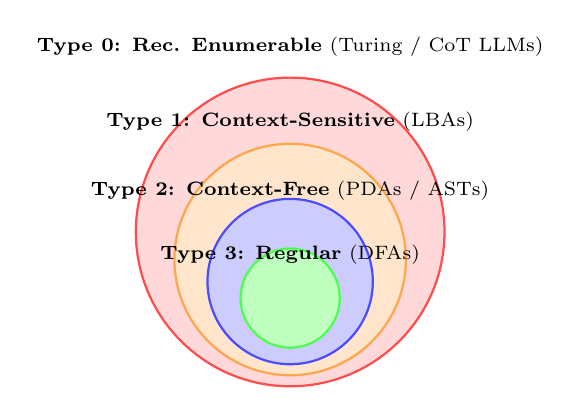
\begin{tikzpicture}[scale=0.7]
            \draw[fill=red!15, draw=red!70, thick] (0,0) circle (2.8cm) node[above=2.1cm] {\scriptsize\textbf{Type 0: Rec. Enumerable} (Turing / CoT LLMs)};
            \draw[fill=orange!20, draw=orange!70, thick] (0,-0.5) circle (2.1cm) node[above=1.5cm] {\scriptsize\textbf{Type 1: Context-Sensitive} (LBAs)};
            \draw[fill=blue!20, draw=blue!70, thick] (0,-0.9) circle (1.5cm) node[above=0.9cm] {\scriptsize\textbf{Type 2: Context-Free} (PDAs / ASTs)};
            \draw[fill=green!25, draw=green!70, thick] (0,-1.2) circle (0.9cm) node[above=0.3cm] {\scriptsize\textbf{Type 3: Regular} (DFAs)};
        \end{tikzpicture}
        \end{center}
        
        \column{0.46\textwidth}
        \begin{alertblock}{Key Empirical Findings}
            \begin{itemize}\small
                \item Standard Transformers without memory fail to generalize on non-regular languages ($a^n b^n c^n$).
                \item Memory-augmented neural models track the Chomsky hierarchy with mathematical precision!
            \end{itemize}
        \end{alertblock}
    \end{columns}
\end{frame}

% ==============================================================================
\section{Week 2: Deterministic Finite Automata (DFAs)}
% ==============================================================================

\begin{frame}{Week 2: Deterministic Finite Automata (DFA)}
    \begin{block}{Formal Definition (Sipser Def 1.5)}
        A \textbf{Deterministic Finite Automaton (DFA)} is a 5-tuple $(Q, \Sigma, \delta, q_0, F)$:
        \begin{enumerate}
            \item $Q$ is a finite set of \textbf{states}.
            \item $\Sigma$ is a finite set of symbols (\textbf{alphabet}).
            \item $\delta: Q \times \Sigma \to Q$ is the \textbf{transition function}.
            \item $q_0 \in Q$ is the \textbf{start state}.
            \item $F \subseteq Q$ is the set of \textbf{accept (final) states}.
        \end{enumerate}
    \end{block}
    
    \begin{exampleblock}{DFA State Diagram: Strings ending with '1'}
        \centering
        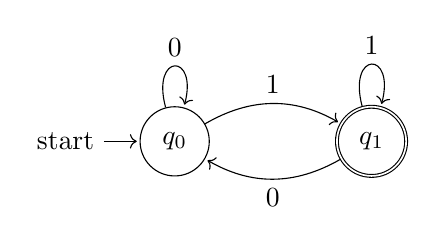
\begin{tikzpicture}[shorten >=1pt, node distance=2.5cm, on grid, auto]
           \node[state, initial] (q0)   {$q_0$}; 
           \node[state, accepting] (q1) [right=of q0] {$q_1$}; 
            \path[->] 
            (q0) edge [loop above] node {0} ()
                 edge [bend left]  node {1} (q1)
            (q1) edge [loop above] node {1} ()
                 edge [bend left]  node {0} (q0);
        \end{tikzpicture}
    \end{exampleblock}
\end{frame}

\begin{frame}{Week 2 Research Spotlight: High-Speed Deep Packet Inspection}
    \begin{exampleblock}{Seminal Reading: ACM SIGCOMM}
        \textbf{Kumar et al. (Univ. of Wisconsin / Cisco)}, \textit{``Algorithms to Accelerate Multiple Regular Expression Matching for Deep Packet Inspection,''} \textbf{ACM SIGCOMM CCR}.
    \end{exampleblock}
    
    \begin{columns}[T]
        \column{0.48\textwidth}
        \begin{block}{The Hardware Challenge}
            \begin{itemize}
                \item Modern network switches process 100+ Gbps traffic in real time.
                \item Snort and Zeek firewalls must scan every byte against 10,000+ malware signature patterns.
            \end{itemize}
        \end{block}
        
        \column{0.48\textwidth}
        \begin{alertblock}{The DFA Solution: $D^2FA$}
            \begin{itemize}
                \item Hardware-compiled DFAs process each incoming byte in strictly \textbf{1 clock cycle} ($\mathcal{O}(1)$ per character).
                \item Zero packet buffering, zero drops, mathematically optimal throughput!
            \end{itemize}
        \end{alertblock}
    \end{columns}
\end{frame}

% ==============================================================================
\section{Week 3: Nondeterministic Finite Automata (NFAs)}
% ==============================================================================

\begin{frame}{Week 3: Nondeterministic Finite Automata (NFA)}
    \begin{block}{Formal Definition (Sipser Def 1.16)}
        An \textbf{NFA} is a 5-tuple $(Q, \Sigma, \delta, q_0, F)$ where the transition function allows non-deterministic branching and $\varepsilon$-transitions:
        $$\delta: Q \times \Sigma_{\varepsilon} \to \mathcal{P}(Q), \quad \text{where } \Sigma_{\varepsilon} = \Sigma \cup \{\varepsilon\}$$
    \end{block}
    
    \begin{columns}[T]
        \column{0.48\textwidth}
        \begin{exampleblock}{NFA Power \& Simplicity}
            \begin{itemize}
                \item Allows multiple parallel branches of computation.
                \item Accepts if \textit{at least one} branch reaches an accept state.
                \item Exponentially more concise than DFAs for many languages.
            \end{itemize}
        \end{exampleblock}
        
        \column{0.48\textwidth}
        \begin{alertblock}{Theorem: Equivalence (Sipser Thm 1.39)}
            Every NFA has an equivalent DFA!
            $$\text{Language Recognizable by NFA} \equiv \text{Regular Language}$$
            \textbf{Proof Method:} Powerset (Subset) Construction.
        \end{alertblock}
    \end{columns}
\end{frame}

\begin{frame}{Week 3: The Powerset (Subset) Construction}
    \begin{block}{Algorithm: Converting NFA $N=(Q, \Sigma, \delta, q_0, F)$ to DFA $M=(Q', \Sigma, \delta', q_0', F')$}
        \begin{enumerate}\setlength{\itemsep}{3pt}
            \item Set DFA states to the power set: $Q' = \mathcal{P}(Q)$. (If $|Q| = k$, then $|Q'| \le 2^k$).
            \item Start state: $q_0' = E(\{q_0\})$ (where $E(R)$ is the $\varepsilon$-closure of state set $R$).
            \item Transition function: For $R \in Q'$ and $a \in \Sigma$,
            $$\delta'(R, a) = \bigcup_{r \in R} E(\delta(r, a))$$
            \item Accept states: $F' = \{R \in Q' \mid R \cap F \neq \varnothing\}$.
        \end{enumerate}
    \end{block}
\end{frame}

% ==============================================================================
\section{Week 4: Regular Expressions \& Catastrophic ReDoS}
% ==============================================================================

\begin{frame}{Week 4: Regular Expressions \& Kleene's Theorem}
    \begin{block}{Inductive Definition of Regular Expressions (Sipser Def 1.52)}
        $R$ is a regular expression if $R$ is:
        \begin{enumerate}
            \item $a \in \Sigma$, $\varepsilon$, or $\varnothing$ (Atomic base cases).
            \item $(R_1 \cup R_2)$ (\textbf{Union}), $(R_1 \circ R_2)$ (\textbf{Concatenation}), or $(R_1)^*$ (\textbf{Star}).
        \end{enumerate}
    \end{block}
    
    \begin{exampleblock}{Kleene's Theorem}
        $$\text{A language } L \text{ is regular} \iff L \text{ is described by a regular expression} \iff L \text{ is recognized by a DFA/NFA.}$$
    \end{exampleblock}
\end{frame}

\begin{frame}{Week 4 Research Spotlight: USENIX Security 2018 \& ReDoS Vulnerabilities}
    \begin{exampleblock}{Seminal Reading: USENIX Security 2018}
        \textbf{Staicu \& Pradel (TU Darmstadt)}, \textit{``Freezing the Web: A Study of ReDoS Vulnerabilities in JavaScript-based Web Servers,''} \textbf{USENIX Security Symposium 2018}.
    \end{exampleblock}
    
    \begin{columns}[T]
        \column{0.48\textwidth}
        \begin{block}{The Root Cause: Backtracking Engines}
            \begin{itemize}
                \item Python \texttt{re}, Node.js, and Java use recursive backtracking for regex matching.
                \item On pattern \texttt{(a+)+b} and input $a^n$, engine evaluates $2^n$ permutations $\implies$ \textbf{Server CPU freeze!}
            \end{itemize}
        \end{block}
        
        \column{0.48\textwidth}
        \begin{alertblock}{The Automata Fix (Google RE2 / Rust regex)}
            \begin{itemize}
                \item Build an NFA $\to$ DFA on the fly using Thompson's construction.
                \item Guarantees $\mathcal{O}(n)$ linear matching time on all inputs!
            \end{itemize}
        \end{alertblock}
    \end{columns}
\end{frame}

% ==============================================================================
\section{Week 5: Non-regular Languages \& The Pumping Lemma}
% ==============================================================================

\begin{frame}{Week 5: Limits of Finite Automata}
    \begin{columns}[T]
        \column{0.48\textwidth}
        \begin{block}{The Pigeonhole Principle}
            \begin{itemize}
                \item A DFA with $p$ states processing a string of length $n \ge p$ must visit at least one state \textbf{more than once}.
                \item Therefore, the computation contains a \textbf{loop}.
                \item The string segment corresponding to the loop can be ``pumped'' (repeated 0, 2, 3, \ldots times) and must still be accepted!
            \end{itemize}
        \end{block}
        
        \column{0.48\textwidth}
        \begin{center}
        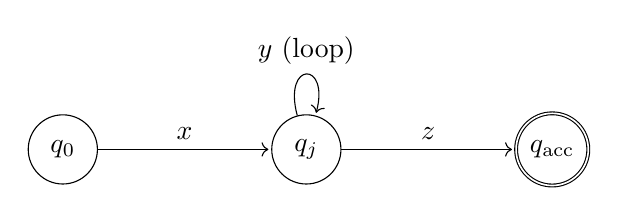
\begin{tikzpicture}[shorten >=1pt, node distance=2.2cm, auto]
           \node[state] (q0) {$q_0$}; 
           \node[state] (q1) [right=of q0] {$q_j$}; 
           \node[state, accepting] (q2) [right=of q1] {$q_{\text{acc}}$}; 
            \path[->] 
            (q0) edge node {$x$} (q1)
            (q1) edge [loop above] node {$y$ (loop)} (q1)
                 edge node {$z$} (q2);
        \end{tikzpicture}
        \end{center}
        \small String $s = xyz$. For any $i \ge 0$, $xy^iz$ must also be accepted.
    \end{columns}
\end{frame}

\begin{frame}{Week 5: The Pumping Lemma for Regular Languages (Sipser Thm 1.70)}
    \begin{block}{Formal Theorem Statement}
        If $L$ is a regular language, then there exists a pumping length $p \ge 1$ such that every string $s \in L$ with $|s| \ge p$ can be divided into $s = xyz$ satisfying:
        \begin{enumerate}
            \item $xy^i z \in L$ for each $i \ge 0$,
            \item $|y| > 0$,
            \item $|xy| \le p$.
        \end{enumerate}
    \end{block}
    
    \begin{alertblock}{Adversarial Game Proof Strategy}
        To prove $L = \{0^n 1^n \mid n \ge 0\}$ is non-regular:
        \begin{enumerate}
            \item \textbf{Assume} $L$ is regular (so $p$ exists).
            \item \textbf{Choose} $s = 0^p 1^p \in L$ ($|s| = 2p \ge p$).
            \item Since $|xy| \le p$, $y$ consists entirely of $0$'s ($y = 0^k, k > 0$).
            \item Pump down with $i=0$: $xy^0z = 0^{p-k} 1^p \notin L$ (fewer $0$'s than $1$'s) $\implies$ \textbf{Contradiction!}
        \end{enumerate}
    \end{alertblock}
\end{frame}

% --- Summary Slide ---
\begin{frame}{Module 1 Summary \& Looking Ahead to Module 2}
    \begin{block}{Key Takeaways}
        \begin{itemize}\setlength{\itemsep}{2pt}
            \item \textbf{DFAs, NFAs, and Regular Expressions} are mathematically equivalent representations of \textbf{Regular Languages}.
            \item Regular languages are strictly limited to problems that require \textbf{finite, bounded memory}.
            \item They cannot count or match arbitrary nested structures ($0^n 1^n$ or balanced parentheses).
        \end{itemize}
    \end{block}
    
    \begin{exampleblock}{Looking Ahead: Module 2 (Context-Free Languages \& Grammars)}
        How do we parse programming languages, arithmetic expressions, and LLM JSON outputs? We add a \textbf{Stack} $\to$ \textbf{Pushdown Automata \& Context-Free Grammars!}
    \end{exampleblock}
\end{frame}

\end{document}
